\subsection{Xây dựng mô-đun dịch Việt - Lào}

Sau khi mô-đun ghép câu trả về câu tiếng Việt hoàn chỉnh, mô-đun dịch Việt - Lào tiếp
nhận chuỗi đó và thực hiện suy luận dịch máy. So với mô-đun ghép câu, phần cài đặt của
mô-đun dịch ngắn hơn, nhưng mỗi bước đều phụ thuộc chặt vào cấu hình của mô hình nền
đa ngôn ngữ và adapter LoRA.

\subsubsection{Các thành phần chính trong mã nguồn}

Trong snapshot hiện tại, mô-đun dịch được tổ chức khá gọn, trọng tâm nằm ở tệp
\texttt{translate.py}. Tệp này chịu trách nhiệm:
\begin{itemize}
    \item nạp tokenizer từ thư mục adapter;
    \item nạp mô hình nền \texttt{facebook/nllb-200-distilled-600M};
    \item ghép adapter LoRA bằng \texttt{PeftModel.from\_pretrained()};
    \item cung cấp hàm \texttt{translate\_vi\_to\_lao(text)} để suy luận;
    \item chạy giao diện dòng lệnh tối giản để thử dịch từng câu.
\end{itemize}

\begin{table}[H]
\centering
\caption{Các thành phần phần mềm chính của mô-đun dịch Việt - Lào}
\begin{tabularx}{\textwidth}{|>{\raggedright\arraybackslash}p{5.2cm}|X|}
\hline
\textbf{Thành phần} & \textbf{Chức năng} \\
\hline
\texttt{translate.py} & Khởi tạo tokenizer, mô hình nền, adapter LoRA và thực hiện suy luận dịch. \\
\hline
\codepath{model/.../adapter_config.json} & Lưu cấu hình LoRA như hạng thấp, dropout và các lớp mục tiêu. \\
\hline
\codepath{model/.../adapter_model.safetensors} & Chứa trọng số adapter đã được fine-tune cho cặp Việt -- Lào. \\
\hline
\codepath{dataset/vi_lo_dataset_split} & Lưu các tập train, validation, test ở dạng CSV. \\
\hline
\end{tabularx}
\end{table}

\subsubsection{Quy trình khởi tạo mô hình}

Khi chương trình bắt đầu, \texttt{translate.py} thực hiện ba bước nạp chính:
\begin{enumerate}
    \item nạp tokenizer từ thư mục adapter cục bộ;
    \item nạp mô hình nền NLLB-200 Distilled 600M;
    \item gắn adapter LoRA vào mô hình nền bằng PEFT.
\end{enumerate}

Việc tách mô hình thành \textit{base model} và \textit{adapter} có hai lợi ích rõ rệt:
\begin{itemize}
    \item giảm kích thước phần cần lưu trữ trong repository;
    \item cho phép thay adapter theo từng tác vụ mà không phải sao chép toàn bộ mô hình
    dịch nền.
\end{itemize}

Về mặt triển khai, đây là một kiến trúc rất phù hợp cho đồ án vì có thể tái sử dụng cùng một
mô hình nền NLLB cho nhiều tác vụ hoặc nhiều cặp ngôn ngữ khác nhau trong tương lai.

\subsubsection{Quy trình suy luận một câu dịch}

Hàm \texttt{translate\_vi\_to\_lao(text)} hiện thực hóa suy luận theo đúng logic của
NLLB:
\begin{itemize}
    \item đặt \texttt{tokenizer.src\_lang = "vie\_Latn"};
    \item mã hóa câu đầu vào thành tensor;
    \item gọi \texttt{model.generate()} với \texttt{forced\_bos\_token\_id} tương ứng
    \texttt{lao\_Laoo};
    \item giới hạn độ dài sinh ở 128 token;
    \item dùng \texttt{num\_beams = 5} để tăng độ ổn định của đầu ra;
    \item giải mã tensor sinh ra thành câu tiếng Lào.
\end{itemize}

Ý nghĩa của cấu hình này là mô hình luôn biết rõ ngôn ngữ nguồn và ngôn ngữ đích trong
quá trình suy luận. Với các mô hình dịch đa ngôn ngữ, đây là điều bắt buộc, vì thiếu token
ngôn ngữ sẽ dễ dẫn đến đầu ra sai ngôn ngữ hoặc pha trộn mã ngôn ngữ không mong muốn.

\begin{figure}[H]
\centering
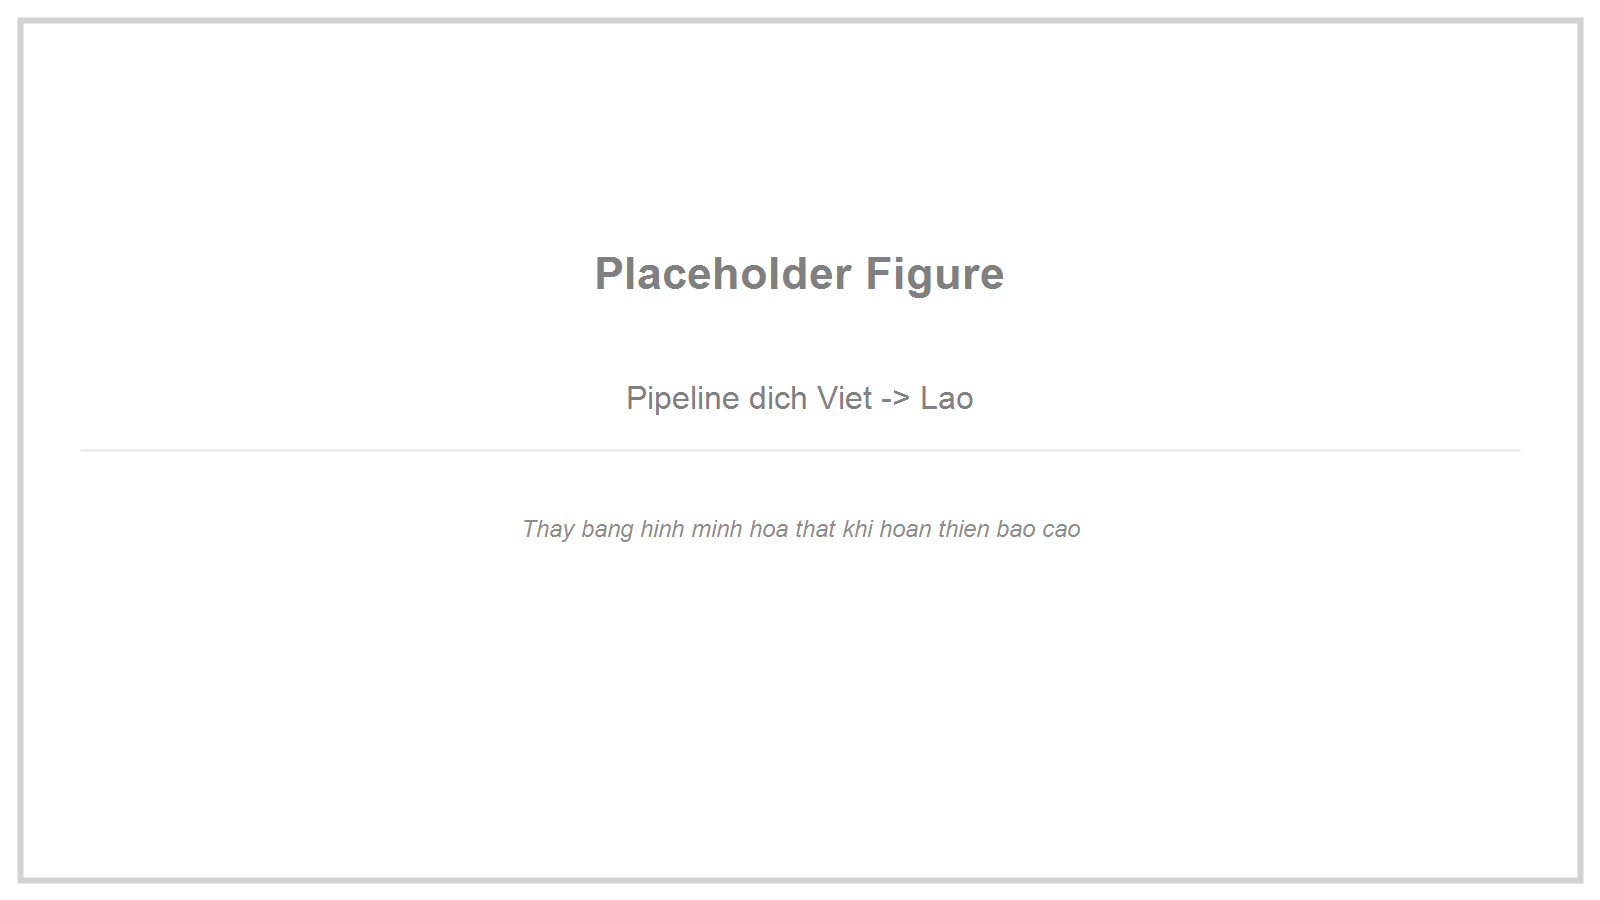
\includegraphics[width=0.86\textwidth]{figures/translation/vi_lao_mt_pipeline.png}
\caption{Luồng cài đặt và suy luận trong mô-đun dịch Việt -- Lào}
\label{fig:translation-runtime}
\end{figure}

\subsubsection{Vai trò của LoRA trong phần mềm}

Mặc dù phần mã gọi LoRA chỉ gồm vài dòng, adapter thực chất là thành phần quan trọng
nhất quyết định việc mô hình nền NLLB có thích nghi được với cặp Việt - Lào hay không.
Trong project này, LoRA được gắn vào các lớp attention projection và lớp đầu ra, tức là
đúng những điểm có ảnh hưởng mạnh đến khả năng căn chỉnh biểu diễn giữa câu nguồn và
câu đích.

So với full fine-tuning, cách làm này mang lại ba lợi ích trực tiếp cho phần mềm:
\begin{itemize}
    \item dễ đóng gói mô hình hơn;
    \item ít rủi ro hơn khi cập nhật mô hình nền;
    \item thuận tiện cho việc thử nhiều adapter khác nhau trên cùng một interface dịch.
\end{itemize}

\subsubsection{Tích hợp với mô-đun ghép câu phía trước}

Mô-đun dịch chỉ thực sự phát huy hiệu quả khi câu tiếng Việt đầu vào đã đủ mạch lạc. Vì
vậy, chất lượng của mô-đun này phụ thuộc mạnh vào đầu ra của mô-đun ghép câu:
\begin{itemize}
    \item nếu câu tiếng Việt rõ chủ-vị và đúng ý nghĩa, NLLB dễ dịch chính xác hơn;
    \item nếu câu tiếng Việt còn thiếu thành phần, dịch máy dễ tạo ra câu tiếng Lào khó
    hiểu hoặc lệch nghĩa;
    \item nếu tầng ghép câu đã chuẩn hóa dấu câu và viết hoa, tokenizer của mô hình dịch
    cũng làm việc ổn định hơn.
\end{itemize}

Nói cách khác, hai mô-đun NLP trong hệ thống không tách rời, mà bổ trợ cho nhau theo
kiểu nối tầng: mô-đun ghép câu giảm nhiễu ngôn ngữ nội bộ, còn mô-đun dịch chuyển ý
nghĩa đó sang ngôn ngữ đích.

\subsubsection{Nhận xét về hiện thực phần mềm}

Điểm mạnh của phần cài đặt hiện tại là đơn giản, rõ ràng và đúng với thực tế nghiên cứu
ứng dụng. Chỉ với một script ngắn, hệ thống đã có thể nạp được mô hình nền đa ngôn ngữ,
adapter tinh chỉnh riêng cho tác vụ và thực hiện suy luận câu mới.

Tuy nhiên, vẫn còn các điểm cần hoàn thiện thêm trong giai đoạn sau:
\begin{itemize}
    \item chưa có script đánh giá full test set đi kèm trực tiếp trong snapshot hiện tại;
    \item chưa có lớp giao tiếp trung gian để gọi mô-đun dịch như một service trong ứng
    dụng lớn hơn;
    \item lần chạy đầu tiên có thể phụ thuộc vào việc mô hình nền đã có cache cục bộ hay
    chưa.
\end{itemize}

Những điểm này không làm sai kiến trúc của mô-đun, nhưng là các hạng mục nên được bổ
sung nếu muốn biến phần nghiên cứu thành sản phẩm phần mềm hoàn chỉnh hơn.

